\section{Design patterns}
\subsection{Chain of Responsibility}\label{Chain of responsibility}
\paragraph{Scopo}
Evitare l'accoppiamento tra il mittente di una richiesta ed il destinatario, in modo che più di un singolo oggetto possa eseguire la richiesta.
Concatenare gli oggetti destinatari e passare la richiesta di oggetto in oggetto, finché uno di questi non riesce ad esaudirla.
\paragraph{Motivazione}
L'oggetto che ha iniziato la richiesta non è a conoscenza di chi la esaudirà, per questo si parla di destinatario implicito.
Ogni oggetto della catena condivide un' interfaccia comune \textit{Handler} per la gestione delle richieste e per accedere al successivo elemento della catena. Questo per consentire il passaggio lungo la catena e per assicurare che l'oggetto che eventualmente esaudirà la richiesta rimanga implicito.
Il metodo che viene mantenuto in tutte le interfacce per creare la catena si chiama \textit{handle}.
\textit{handle}, nella versione standard, esegue la chiamata al successore nella catena. Alla fine della catena viene fatto l'overriding di questo metodo, implementando la richiesta iniziale oppure gestendo l'errore.
\paragraph{Applicabilità}
\textit{Chain of Responsibility} si usa nei seguenti casi:
\begin{itemize}
\item Più di un oggetto può gestire la richiesta ed il ricevente che la gestirà non è conosciuto a priori;
\item Si vuole passare una richiesta ad uno dei molti oggetti, senza esplicitare il ricevente;
\item L'insieme di oggetti che gestirà una richiesta deve essere definito dinamicamente.
\end{itemize}
\paragraph{Utilizzo}
Express usa \textit{Chain of Responsibility} per la gestione dei middleware e del routing. Nell'architettura viene utilizzato all'interno del package \gloxy{Back-End}::App. Ogni \textit{ConcreteHandler} eredita da \textit{MiddlewareHandler}, che corrisponde all'interfaccia astratta \textit{Handler} del Design Pattern.
Con Express i middleware corrispondono ai \textit{ConcreteHandler}. L'implementazione di questi risulta sotto alcuni aspetti differente da una normale implementazione del pattern:
\begin{enumerate}
\item I middleware di Express possono essere delle classi che implementano il metodo \textit{handle} oppure delle funzioni secondo lo stile funzionale delle \gloxy{librerie} e dei moduli di Node.js. Nella nostra architettura abbiamo utilizzato principalmente la seconda versione;
\item Nel \gloxy{Design Pattern} è previsto che l'oggetto \textit{ConcreteHandler} abbia un riferimento (successor) al \textit{ConcreteHandler} successivo. Express, anzichè un riferimento, passa al metodo che esegue il middleware una \gloxy{callback}. Il middleware che esegue la \gloxy{callback} passa il controllo all'oggetto del \gloxy{server} di Express, il quale passerà a sua volta il controllo al successivo middleware.
\end{enumerate}
Express divide i middleware in due tipologie:
\begin{enumerate}
\item \textit{Middleware standard} con 3 parametri formali;
\item \textit{Middleware per la gestione degli errori} con 4 parametri formali, ovvero i 3 del middleware standard più un parametro per gli errori.
\end{enumerate}
Ogni middleware può passare il controllo al middleware standard successivo, oppure ad un middleware per la gestione degli errori, passandogli l'errore relativo.
Ogni middleware di Express deve essere invocato con i parametri  elencati \uline{nel seguente ordine}:
\begin{enumerate}
\item L'eventuale errore da gestire, in caso si tratti di un middleware per la gestione degli errori;
\item L'oggetto contenente la richiesta da risolvere;
\item L'oggetto che conterrà la risposta;
\item La \gloxy{callback} da utilizzare per passare il controllo al successivo middleware.
\end{enumerate}
\paragraph{Struttura}
\begin{center}
\begin{figure}[h]
\centering
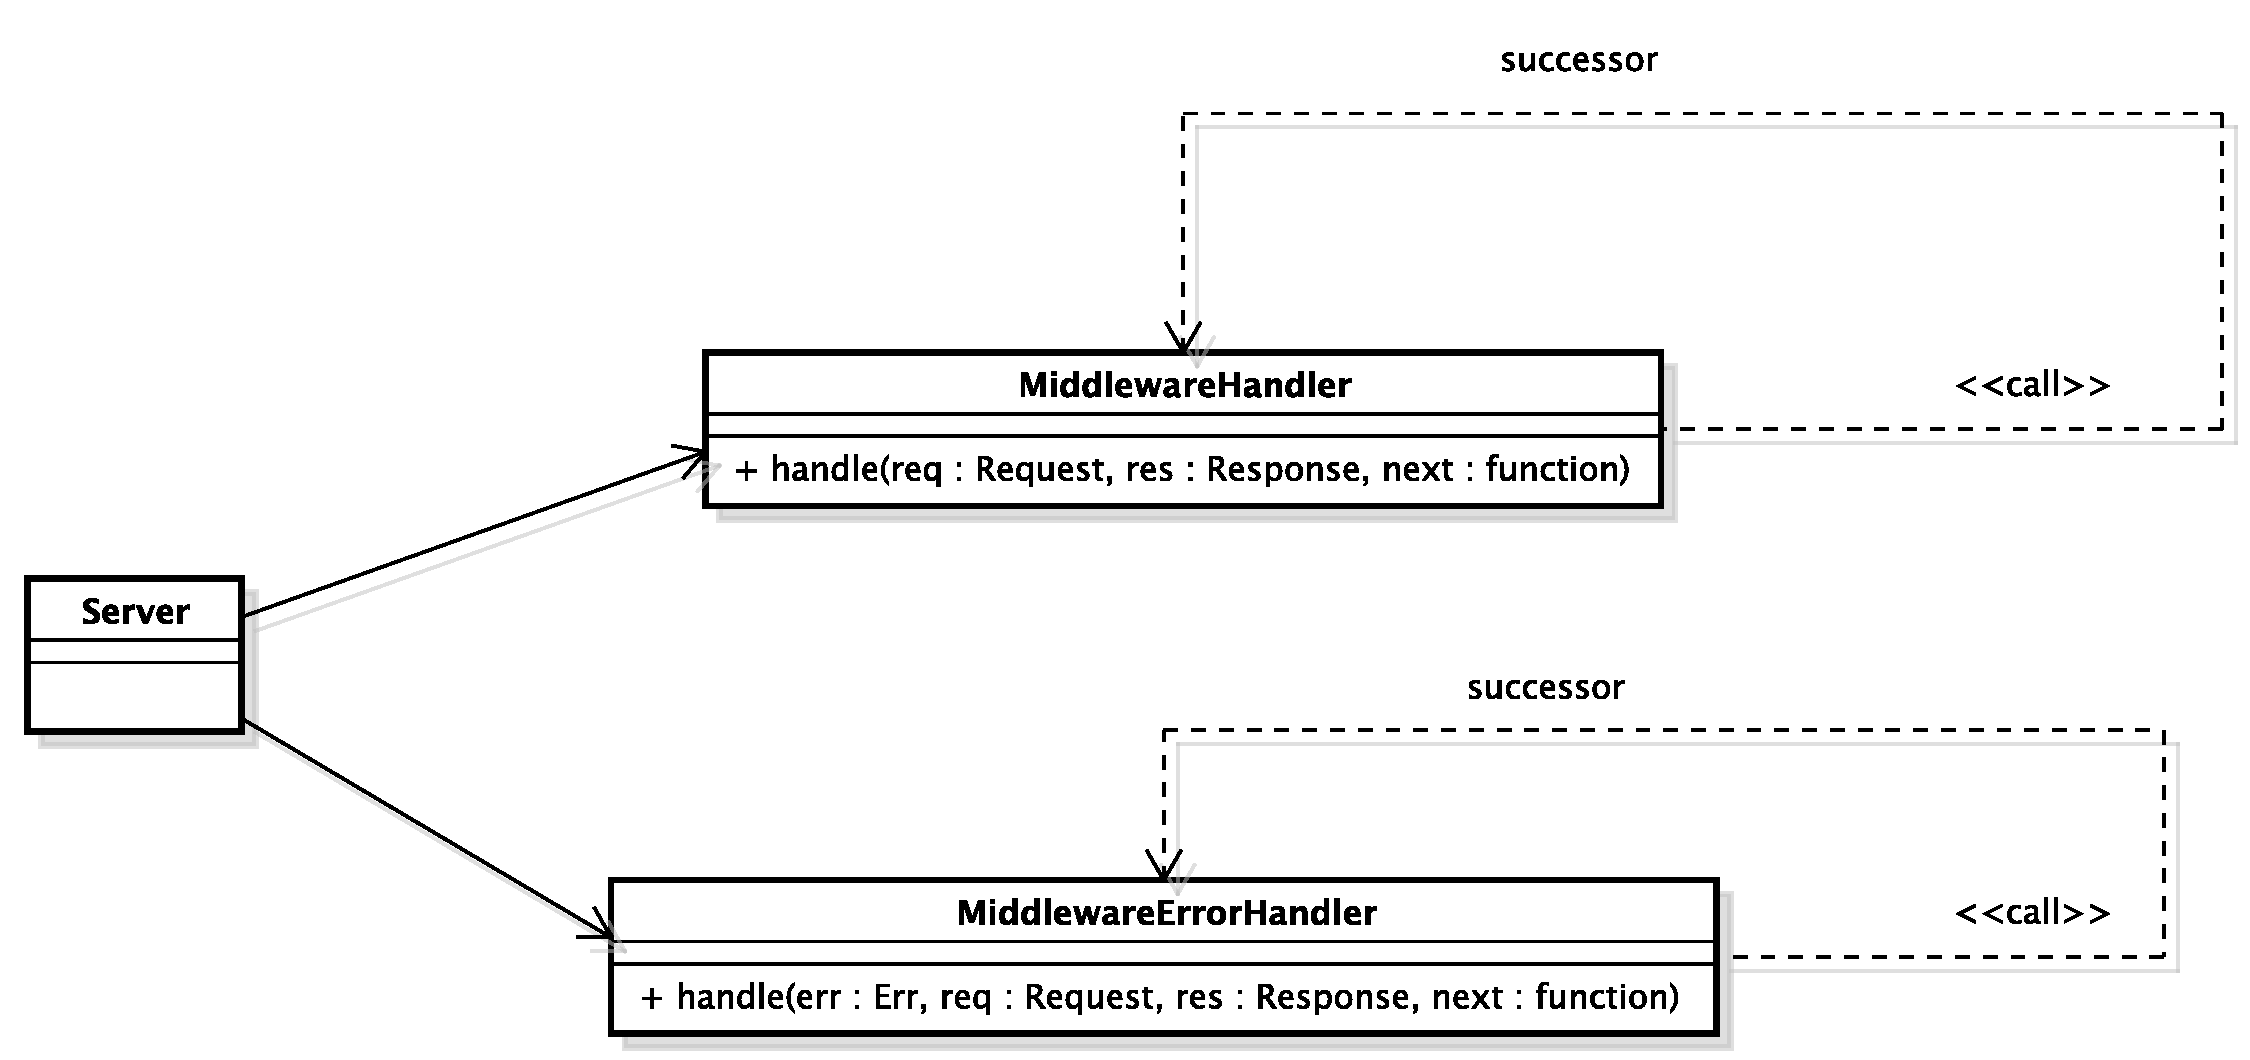
\includegraphics[scale=0.33,keepaspectratio]{diagrammi/designPatterns/ChainOfPremi.pdf}\label{chainOfPremi}
\caption{Chain Of Responsibility contestualizzato}
\end{figure}
\FloatBarrier
\end{center}
\paragraph{Collaborazioni}
Quando un \gloxy{client} effettua una richiesta, questa viene propagata lungo la catena finché un \textit{ConcreteHandler} non si assume la responsabilità di gestirla.
\paragraph{Svantaggi}
\`E necessario porre attenzione a come si configura la catena. Infatti, in caso di configurazione inappropriata, sussiste il rischio che la richiesta passi per diversi punti della catena senza essere mai realizzata, oppure che la richiesta non non venga realizzata perché non esiste un \textit{ConcreteHandler} che la possa risolvere.
%Se la catena di richieste non è configurata in modo appropriato, c'è il rischio che la richiesta passi per diversi punti della catena senza essere mai realizzata. Oppure è possibile che la richiesta non non venga realizzata perché non esiste un \textit{ConcreteHandler} che la possa risolvere.
\subsection{Dependecy Injection}\label{Dependency Injection}
\paragraph{Scopo}
%Evitare di inserire all'interno delle componenti il codice che si occupa di risolvere le dipendenze con le altre componenti dell'applicazione.
Separare il codice della componente dal codice che si occupa di risolvere le dipendenze con le altre componenti.
\paragraph{Motivazione}
%Lasciando al componente il compito di risolvere le proprie dipendenze, creandosi gli oggetti necessari al suo funzionamento, aumenta l'accoppiamento tra le componenti e rende più difficoltoso progettare i test di unità.
Lasciare al componente il compito di risolvere le proprie dipendenze, creando gli oggetti necessari al suo funzionamento, aumenta l'accoppiamento tra le componenti e rende più difficoltoso progettare i test di unità.\\
Con questo pattern invece è possibile esprimere le dipendenze in modo dichiarativo e utilizzare un oggetto \textit{contenitore} per risolverle dinamicamente a \gloxy{runtime}. In questo modo è possibile scegliere anche quale componente iniettare in base allo stato del programma.\\
\paragraph{Applicabilità}
Questo pattern viene utilizzato dalla maggior parte dei \gloxy{framework} moderni. In particolare, \gloxy{AngularJS} offre il servizio \texttt{\$injector} che permette di invocare delle funzioni iniettando al loro interno degli oggetti.
\paragraph{Struttura}
I componenti coinvolti nel \textit{Dependency Injection} sono:
\begin{itemize}
\item Un \textit{\gloxy{client}} che viene creato e riceve le dipendenze;
\item Un \textit{contenitore} che si occupa di creare il \gloxy{client} e di iniettarvi le dipendenze;
\item Un \textit{servizio} che deve essere iniettato al \gloxy{client}.
\end{itemize}
Nello specifico di \gloxy{AngularJS} \texttt{\$injector} funziona da \textit{contenitore} che si occupa di risolvere le dipendenze. I \textit{\gloxy{client}} sono rappresentati dalle funzioni che costruiscono i componenti dell'applicazione, tipicamente \gloxy{controller} o service. Il \textit{servizio} è un oggetto service che può essere definito dall'utente oppure uno di quelli resi disponibili da \gloxy{AngularJS}.\\
\begin{center}
\begin{figure}[h]
\centering
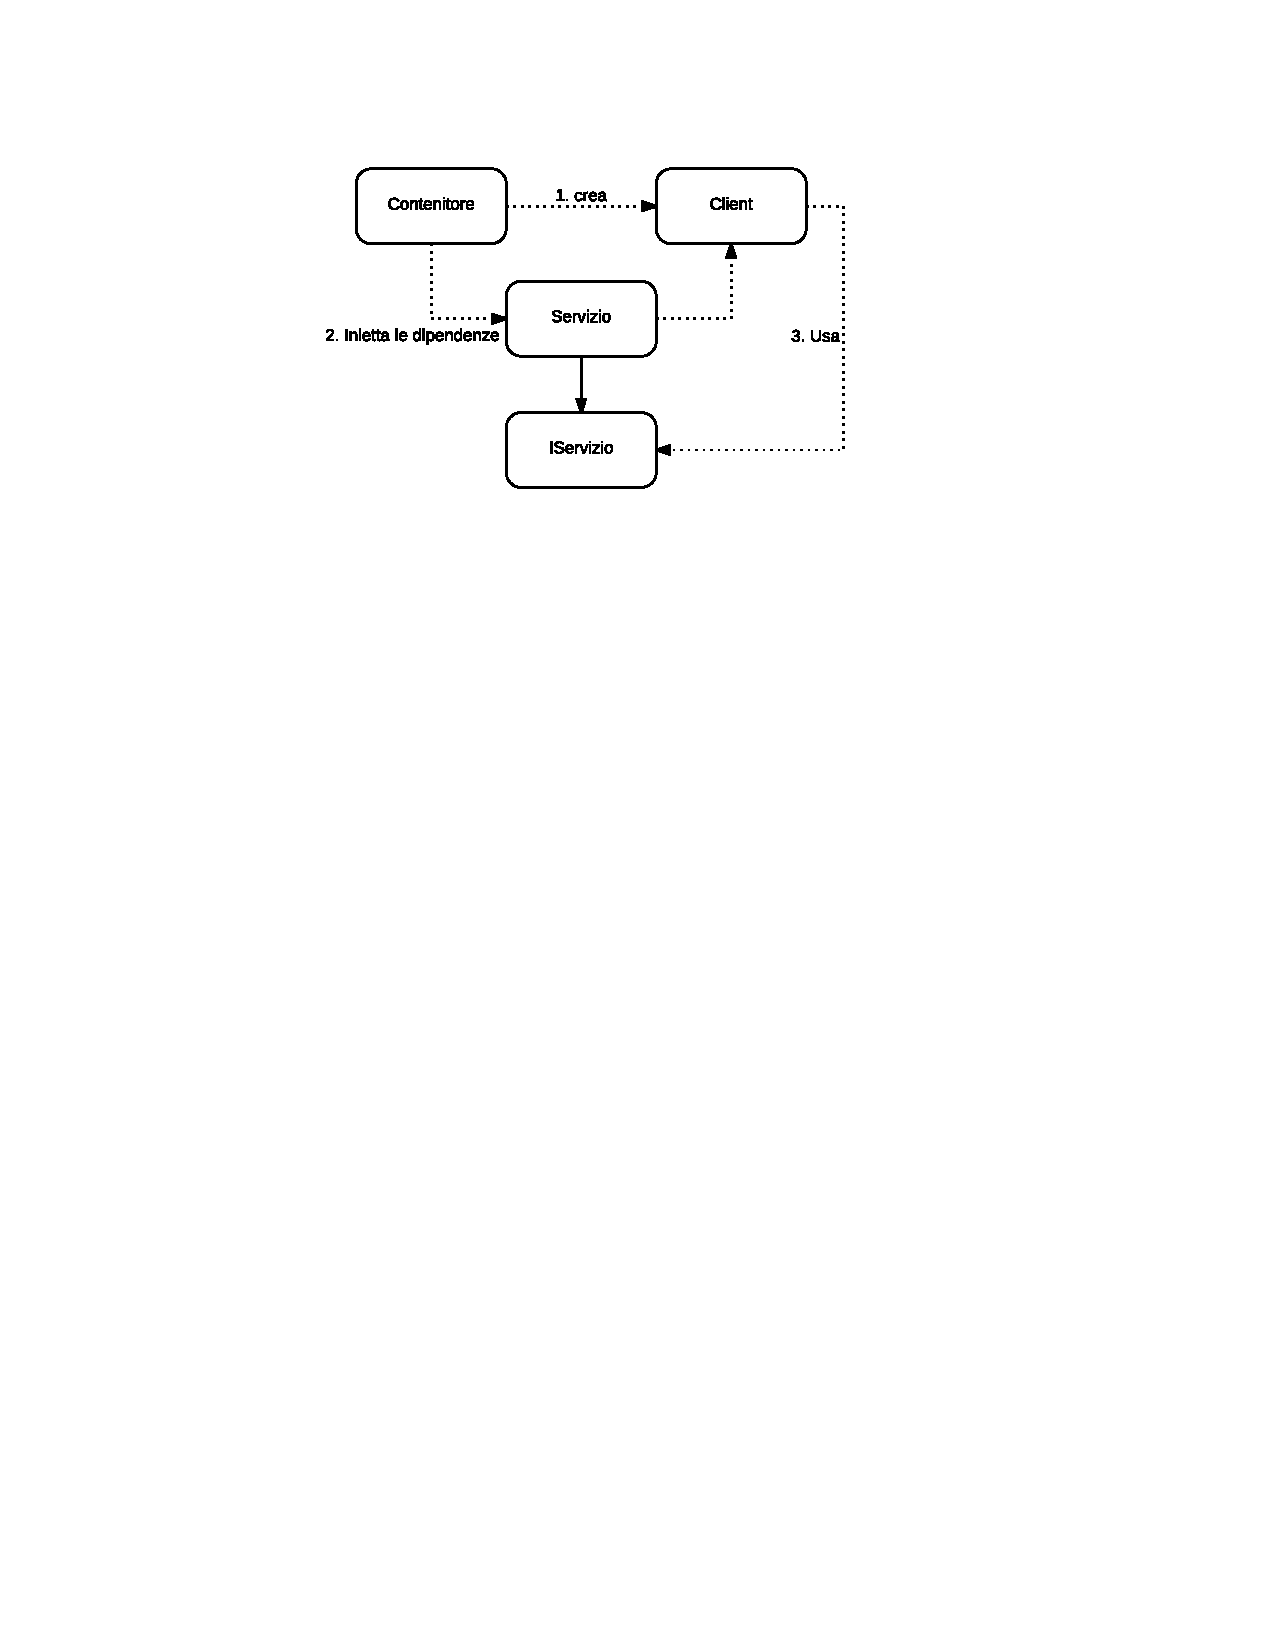
\includegraphics[scale=1,keepaspectratio]{diagrammi/designPatterns/dependencyInjection.pdf}
\caption{Struttura logica del Dependency Injection}
\end{figure}
\FloatBarrier
\end{center}
L'\textit{injection} delle dipendenze può essere fatta in due modi:
\begin{itemize}
\item \textbf{Constructor Injection}: le dipendenze vengono dichiarate come parametri del costruttore che il \textit{container} andrà a valorizzare quando crea l'oggetto. In questo modo l'oggetto costruito è subito utilizzabile e non è mai in uno stato inconsistente. Tuttavia si rende necessario avere dei costruttori con un elevato numero di parametri, che potrebbero rendere i costruttori difficili da comprendere. \gloxy{AngularJS} usa questo tipo di \textit{dependency injection};
\item \textbf{Setter Injection}: le dipendenze vengono dichiarate come metodi \textit{setter} del componente. Questa soluzione è meno ambigua, funziona bene con le gerarchie di classi e non soffre del \textit{telescoping} dei costruttori. Non è però possibile avere oggetti immutabili. \`E possibile che la componente rimanga in uno stato inconsistente, in quanto deve essere costruita per passi.
\end{itemize}
\paragraph{Svantaggi}
Eventuali errori legati alla risoluzione delle dipendenze o alla loro implementazione vengono rilevati solamente a \gloxy{runtime}.
\subsection{Facade}\label{Facade}
\paragraph{Scopo}
Fornire un'interfaccia unica per un sottosistema complesso. Rendere una \gloxy{libreria} più facile da capire, usare e testare. Diminuire le dipendenze tra sottosistemi senza nascondere le funzionalità di basso livello.
\paragraph{Motivazione}
Quando un sistema complesso viene strutturato in sottosistemi, le dipendenze tra essi possono aumentare. Applicare il pattern \gloxy{Facade} in un sottosistema aiuta a diminuire le dipendenze dall'esterno verso le classi che lo compongono. Il sottosistema possederà un'interfaccia semplificata che il \gloxy{client} può utilizzare anziché dover gestire numerosi oggetti. Utilizzare il pattern \gloxy{Facade} promuove un accoppiamento debole tra un sottosistema ed i \gloxy{client}, che comporta una maggiore flessibilità nello sviluppo: è possibile modificare il sottosistema senza che i \gloxy{client} debbano adeguarsi a loro volta.\\
Ciononostante i \gloxy{client} possono comunque accedere alle funzionalità di basso livello ed utilizzare le classi del sottosistema.
\paragraph{Applicabilità}
\textit{\gloxy{Facade}} si usa nei seguenti casi:
\begin{itemize}
\item Si vuole fornire una singola interfaccia semplice per un sottosistema complesso;
\item Si vuole promuovere il disaccoppiamento tra sottosistemi e \gloxy{client}, semplificando le dipendenze;
\item Si vuole stratificare un sistema: è possibile definire una classe \gloxy{Facade} come punto d'ingresso per ogni livello di sottosistema. In questo modo, se vi sono dipendenze fra sottosistemi, essi possono comunicare fra loro attraverso la propria \gloxy{Facade}.
\end{itemize}
\paragraph{Utilizzo}
Nel package \texttt{\nameref{Premi::Back-End::App::Models}} è stata definita una classe \gloxy{Facade} \texttt{\nameref{Premi::Back-End::App::Models::ProjectModel}}. Essa rappresenta un \gloxy{progetto} contenente nodi, relazioni e \gloxy{percorsi di presentazione} e  fornisce un'interfaccia per le classi del package che compongono la mappa mentale. I \gloxy{controller} non dovranno quindi interagire direttamente con gli oggetti di questo package, ma utilizzeranno un'interfaccia unica per: inserire, modificare ed eliminare nodi della mappa mentale, relazioni e \gloxy{percorsi} di presentazione. La classe \texttt{ProjectModel} nasconde inoltre ai \gloxy{controller} la complessità di alcune operazioni. Ad esempio, se si intende rimuovere un nodo della \gloxy{mappa mentale} che risulta padre di un sottoalbero, è necessario eliminare in ricorsione anche i nodi figli. Questa operazione sarebbe particolarmente costosa e renderebbe molto complesso il codice del \gloxy{controller}.\\
Nel diagramma seguente sono stati tralasciati volontariamente alcuni metodi delle classe, per mostrare in modo semplice e diretto come il pattern è stato applicato.\\
\begin{center}
\begin{figure}[h]
\centering
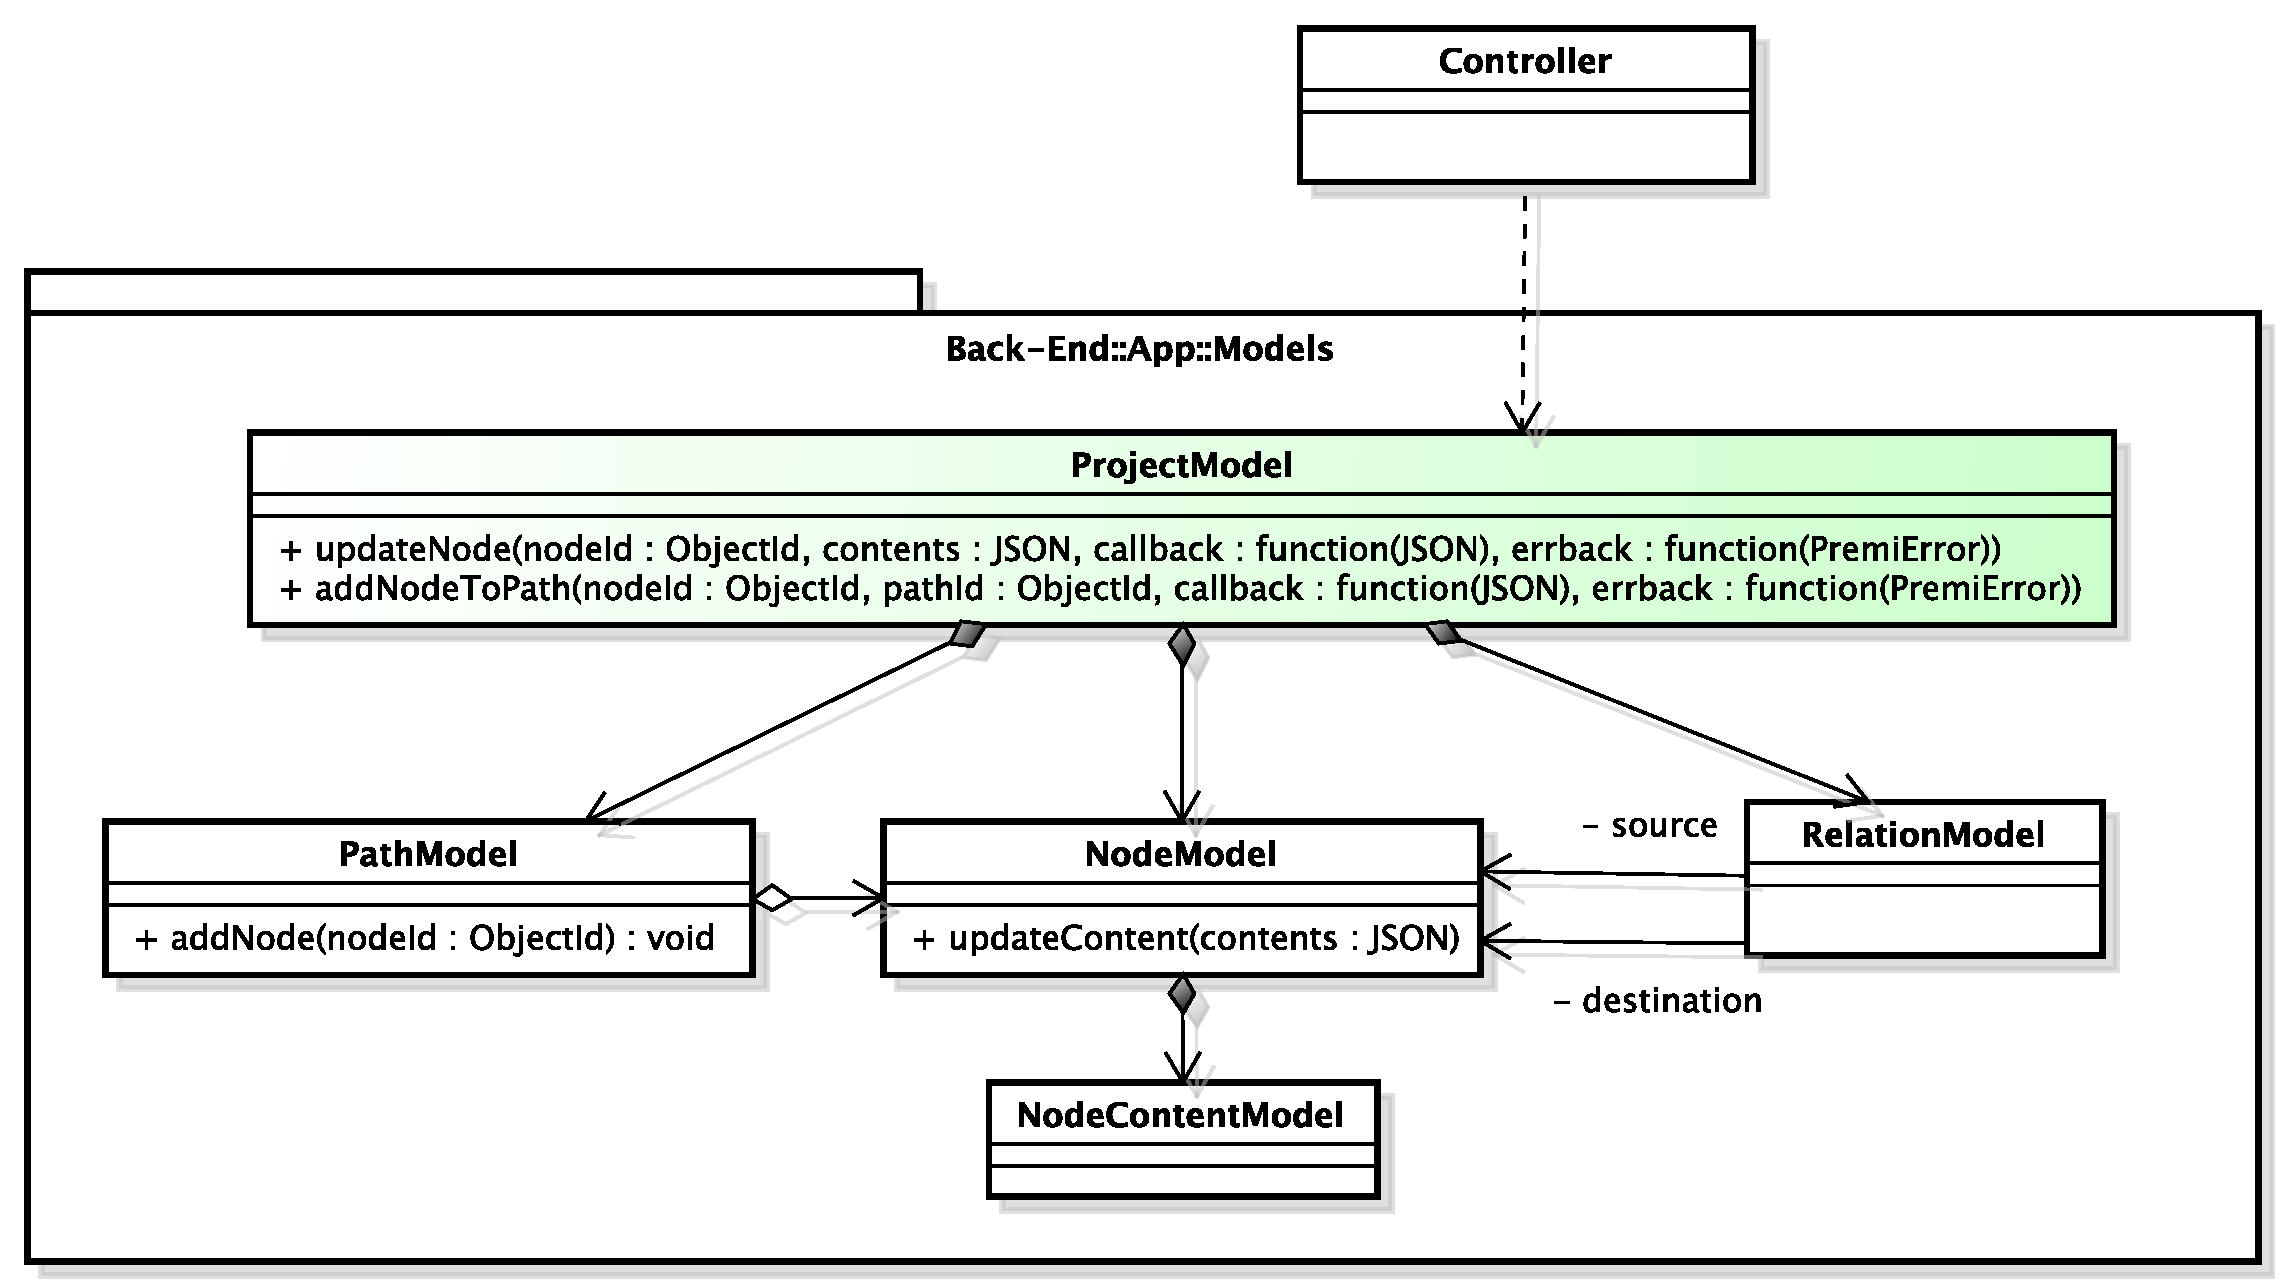
\includegraphics[scale=0.33,keepaspectratio]{diagrammi/designPatterns/facade.pdf}
\caption{Facade contestualizzato}
\end{figure}
\FloatBarrier
\end{center}
\subsection{Observer}\label{Observer}
\paragraph{Scopo}
Permettere a degli oggetti di tenere sotto controllo lo stato di altri oggetti e di essere notificati quando gli oggetti osservati vengono modificati.
\paragraph{Motivazione}
In alcuni casi è necessario è necessario tenere sincronizzati vari oggetti e, nel caso un oggetto venga modificato, avere la possibilità di riflettere il cambiamento sugli altri oggetti dipendenti. \\
Il pattern \gloxy{Observer} permette di implementare ciò definendo due tipologie di oggetti: i \textit{subject}, che rappresentano gli oggetti osservati, e gli \textit{\gloxy{observer}} che rappresentano gli oggetti che osservano lo stato del \texttt{subject}.
Con questo pattern è possibile quindi realizzare un sistema \textit{publish-subscribe}, nel quale i vari \textit{subject} si registrano per essere notificati delle modifiche subite dal \textit{subject}.\\
\paragraph{Applicabilità}
\textit{\gloxy{Observer}} si usa nei seguenti casi:
\begin{itemize}
\item Si vuole che il cambiamento dello stato di un oggetto provochi l'aggiornamento di altri oggetti;
\item Si vuole notificare degli oggetti dell'avvenimento di un determinato evento senza sapere il loro tipo.
\end{itemize}
\paragraph{Utilizzo}
Nella parte \gloxy{front-end} dell'applicazione viene utilizzato per permettere ai vari controllers di essere notificati degli eventi sollevati dalla \gloxy{libreria} Cytoscape.js. Questi eventi infatti non vengono rilevati automaticamente da \gloxy{Angular}, pertanto viene utilizzato il service \texttt{MindmapAdapterService} per creare un livello intermedio che permette di notificare alle altre classi il verificarsi degli eventi di Cytoscape.
L'implementazione avviene memorizzando all'interno di \texttt{MindmapAdapterService} un'array di funzioni da invocare quando si verifica un determinato evento di Cytoscape. Il service fornisce inoltre due metodi che permettono ai \gloxy{controller} di associare e dissociare una funzione che deve essere invocata al verificarsi di un evento.
Questa particolare implementazione è possibile dal momento che le funzioni in \gloxy{JavaScript} vengono trattate come un oggetto qualsiasi.
Segue un diagramma semplificato che illustra come è stato applicato il pattern.\\
\begin{center}
\begin{figure}[h]
\centering
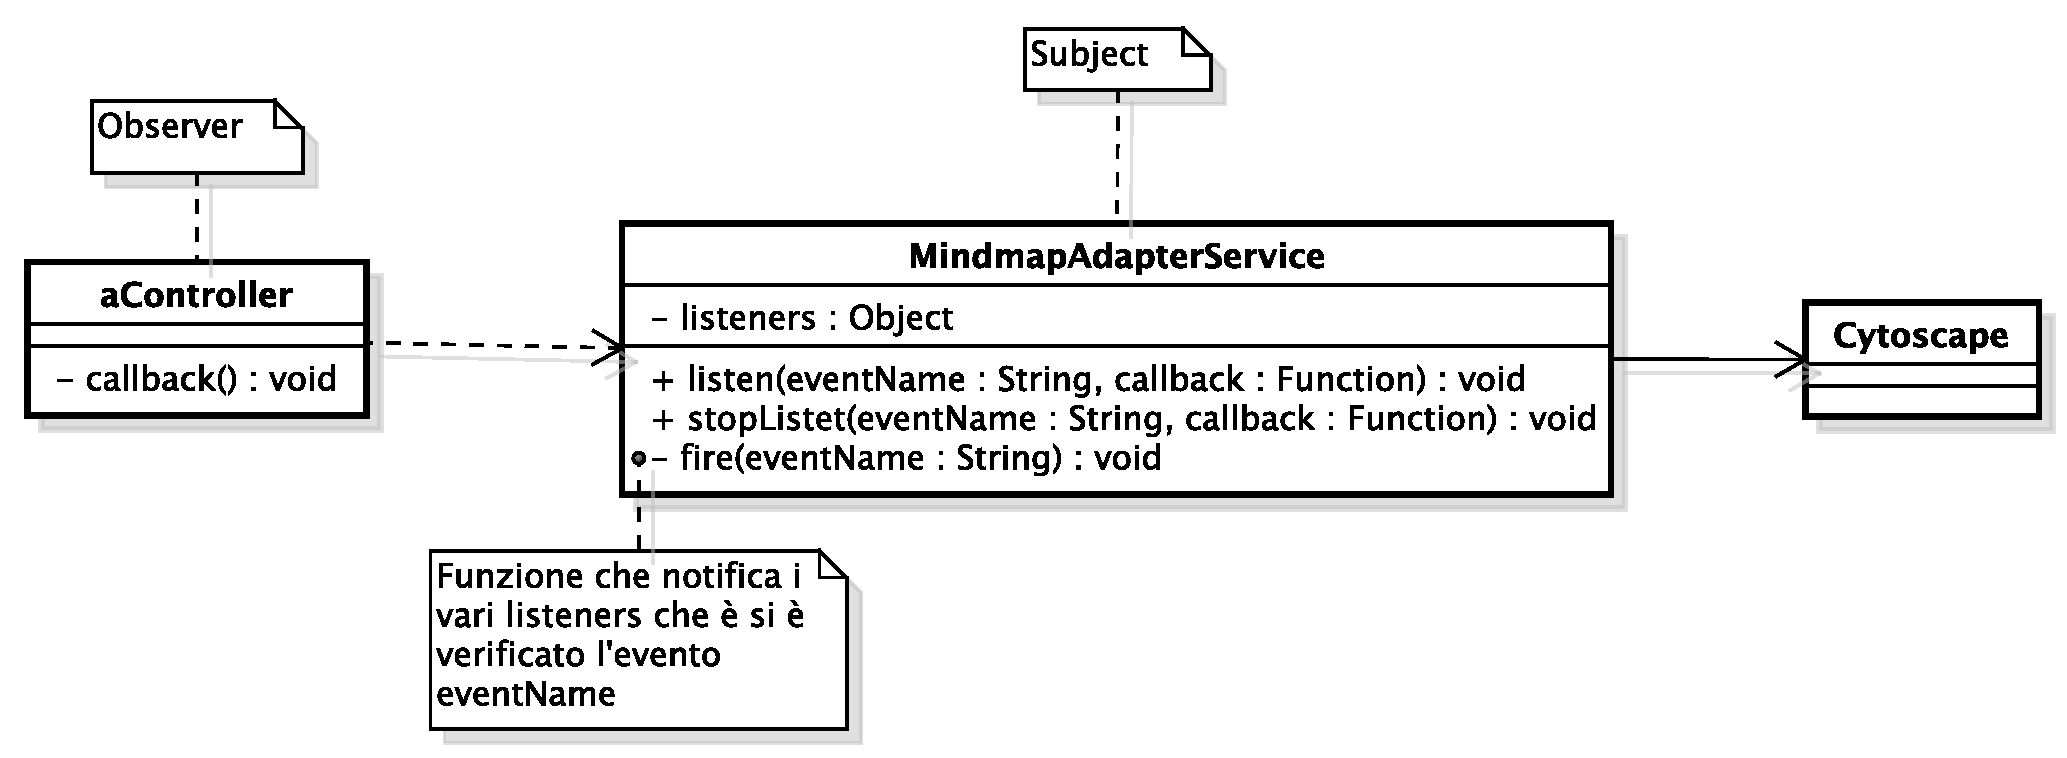
\includegraphics[scale=0.33,keepaspectratio]{diagrammi/designPatterns/observer.pdf}
\caption{Observer contestualizzato}
\end{figure}
\FloatBarrier
\end{center}
